% Options for packages loaded elsewhere
\PassOptionsToPackage{unicode}{hyperref}
\PassOptionsToPackage{hyphens}{url}
%
\documentclass[
]{article}
\title{mSigHdp vignette}
\author{ML and SGR}
\date{06/01/2022}

\usepackage{amsmath,amssymb}
\usepackage{lmodern}
\usepackage{iftex}
\ifPDFTeX
  \usepackage[T1]{fontenc}
  \usepackage[utf8]{inputenc}
  \usepackage{textcomp} % provide euro and other symbols
\else % if luatex or xetex
  \usepackage{unicode-math}
  \defaultfontfeatures{Scale=MatchLowercase}
  \defaultfontfeatures[\rmfamily]{Ligatures=TeX,Scale=1}
\fi
% Use upquote if available, for straight quotes in verbatim environments
\IfFileExists{upquote.sty}{\usepackage{upquote}}{}
\IfFileExists{microtype.sty}{% use microtype if available
  \usepackage[]{microtype}
  \UseMicrotypeSet[protrusion]{basicmath} % disable protrusion for tt fonts
}{}
\makeatletter
\@ifundefined{KOMAClassName}{% if non-KOMA class
  \IfFileExists{parskip.sty}{%
    \usepackage{parskip}
  }{% else
    \setlength{\parindent}{0pt}
    \setlength{\parskip}{6pt plus 2pt minus 1pt}}
}{% if KOMA class
  \KOMAoptions{parskip=half}}
\makeatother
\usepackage{xcolor}
\IfFileExists{xurl.sty}{\usepackage{xurl}}{} % add URL line breaks if available
\IfFileExists{bookmark.sty}{\usepackage{bookmark}}{\usepackage{hyperref}}
\hypersetup{
  pdftitle={mSigHdp vignette},
  pdfauthor={ML and SGR},
  hidelinks,
  pdfcreator={LaTeX via pandoc}}
\urlstyle{same} % disable monospaced font for URLs
\usepackage[margin=1in]{geometry}
\usepackage{color}
\usepackage{fancyvrb}
\newcommand{\VerbBar}{|}
\newcommand{\VERB}{\Verb[commandchars=\\\{\}]}
\DefineVerbatimEnvironment{Highlighting}{Verbatim}{commandchars=\\\{\}}
% Add ',fontsize=\small' for more characters per line
\usepackage{framed}
\definecolor{shadecolor}{RGB}{248,248,248}
\newenvironment{Shaded}{\begin{snugshade}}{\end{snugshade}}
\newcommand{\AlertTok}[1]{\textcolor[rgb]{0.94,0.16,0.16}{#1}}
\newcommand{\AnnotationTok}[1]{\textcolor[rgb]{0.56,0.35,0.01}{\textbf{\textit{#1}}}}
\newcommand{\AttributeTok}[1]{\textcolor[rgb]{0.77,0.63,0.00}{#1}}
\newcommand{\BaseNTok}[1]{\textcolor[rgb]{0.00,0.00,0.81}{#1}}
\newcommand{\BuiltInTok}[1]{#1}
\newcommand{\CharTok}[1]{\textcolor[rgb]{0.31,0.60,0.02}{#1}}
\newcommand{\CommentTok}[1]{\textcolor[rgb]{0.56,0.35,0.01}{\textit{#1}}}
\newcommand{\CommentVarTok}[1]{\textcolor[rgb]{0.56,0.35,0.01}{\textbf{\textit{#1}}}}
\newcommand{\ConstantTok}[1]{\textcolor[rgb]{0.00,0.00,0.00}{#1}}
\newcommand{\ControlFlowTok}[1]{\textcolor[rgb]{0.13,0.29,0.53}{\textbf{#1}}}
\newcommand{\DataTypeTok}[1]{\textcolor[rgb]{0.13,0.29,0.53}{#1}}
\newcommand{\DecValTok}[1]{\textcolor[rgb]{0.00,0.00,0.81}{#1}}
\newcommand{\DocumentationTok}[1]{\textcolor[rgb]{0.56,0.35,0.01}{\textbf{\textit{#1}}}}
\newcommand{\ErrorTok}[1]{\textcolor[rgb]{0.64,0.00,0.00}{\textbf{#1}}}
\newcommand{\ExtensionTok}[1]{#1}
\newcommand{\FloatTok}[1]{\textcolor[rgb]{0.00,0.00,0.81}{#1}}
\newcommand{\FunctionTok}[1]{\textcolor[rgb]{0.00,0.00,0.00}{#1}}
\newcommand{\ImportTok}[1]{#1}
\newcommand{\InformationTok}[1]{\textcolor[rgb]{0.56,0.35,0.01}{\textbf{\textit{#1}}}}
\newcommand{\KeywordTok}[1]{\textcolor[rgb]{0.13,0.29,0.53}{\textbf{#1}}}
\newcommand{\NormalTok}[1]{#1}
\newcommand{\OperatorTok}[1]{\textcolor[rgb]{0.81,0.36,0.00}{\textbf{#1}}}
\newcommand{\OtherTok}[1]{\textcolor[rgb]{0.56,0.35,0.01}{#1}}
\newcommand{\PreprocessorTok}[1]{\textcolor[rgb]{0.56,0.35,0.01}{\textit{#1}}}
\newcommand{\RegionMarkerTok}[1]{#1}
\newcommand{\SpecialCharTok}[1]{\textcolor[rgb]{0.00,0.00,0.00}{#1}}
\newcommand{\SpecialStringTok}[1]{\textcolor[rgb]{0.31,0.60,0.02}{#1}}
\newcommand{\StringTok}[1]{\textcolor[rgb]{0.31,0.60,0.02}{#1}}
\newcommand{\VariableTok}[1]{\textcolor[rgb]{0.00,0.00,0.00}{#1}}
\newcommand{\VerbatimStringTok}[1]{\textcolor[rgb]{0.31,0.60,0.02}{#1}}
\newcommand{\WarningTok}[1]{\textcolor[rgb]{0.56,0.35,0.01}{\textbf{\textit{#1}}}}
\usepackage{graphicx}
\makeatletter
\def\maxwidth{\ifdim\Gin@nat@width>\linewidth\linewidth\else\Gin@nat@width\fi}
\def\maxheight{\ifdim\Gin@nat@height>\textheight\textheight\else\Gin@nat@height\fi}
\makeatother
% Scale images if necessary, so that they will not overflow the page
% margins by default, and it is still possible to overwrite the defaults
% using explicit options in \includegraphics[width, height, ...]{}
\setkeys{Gin}{width=\maxwidth,height=\maxheight,keepaspectratio}
% Set default figure placement to htbp
\makeatletter
\def\fps@figure{htbp}
\makeatother
\setlength{\emergencystretch}{3em} % prevent overfull lines
\providecommand{\tightlist}{%
  \setlength{\itemsep}{0pt}\setlength{\parskip}{0pt}}
\setcounter{secnumdepth}{-\maxdimen} % remove section numbering
\ifLuaTeX
  \usepackage{selnolig}  % disable illegal ligatures
\fi

\begin{document}
\maketitle

`

This vignette is to introduce how to use mSigHdp (Liu et al., 2021)

\begin{Shaded}
\begin{Highlighting}[]
\NormalTok{devtools}\SpecialCharTok{::}\FunctionTok{install\_github}\NormalTok{(}\StringTok{"steverozen/mSigHdp"}\NormalTok{,}\AttributeTok{ref=}\StringTok{"master"}\NormalTok{)}
\end{Highlighting}
\end{Shaded}

\hypertarget{toy-dataset}{%
\section{Toy dataset}\label{toy-dataset}}

To illustrate the basic features of the mSigHdp package, we consider a
toy data set of categorical count data with \textbf{10 samples} (rows)
and \textbf{96 categories} (columns). The \textbf{10 samples} are PCAWG
platinum tumors

\begin{Shaded}
\begin{Highlighting}[]
\FunctionTok{library}\NormalTok{(mSigHdp)}
\NormalTok{toy\_data }\OtherTok{\textless{}{-}}\NormalTok{ ICAMS}\SpecialCharTok{::}\FunctionTok{ReadCatalog}\NormalTok{(}\StringTok{"toy\_data.csv"}\NormalTok{)}
\end{Highlighting}
\end{Shaded}

Run Runhdpxparallel to extract signatures from toy data set. There are
three checkpoint arguments: checkpoint.chlist to checkpoint the chlist
to ``initial.chlist.Rdata'' in the current working directory.
checkpoint.1.chain to checkpoint the sample chain to current working
directory, posterior.checkpoint to checkpoint the posterior sampling
after every 10 posterior samples collected.

\begin{Shaded}
\begin{Highlighting}[]
\NormalTok{retval }\OtherTok{\textless{}{-}}\NormalTok{ mSigHdp}\SpecialCharTok{::}\FunctionTok{RunHdpxParallel}\NormalTok{(}\AttributeTok{input.catalog =}\NormalTok{ toy\_data,}
                          \AttributeTok{out.dir                  =} \StringTok{"vignettes"}\NormalTok{,}
                          \AttributeTok{num.child.process        =} \DecValTok{4}\NormalTok{, }
                          \AttributeTok{CPU.cores                =} \DecValTok{4}\NormalTok{,}
                          \AttributeTok{seedNumber               =} \DecValTok{123}\NormalTok{,}
                          \AttributeTok{K.guess                  =} \DecValTok{5}\NormalTok{,}
                          \AttributeTok{burnin.checkpoint        =} \ConstantTok{FALSE}\NormalTok{,}
                          \AttributeTok{burnin                   =} \DecValTok{100}\NormalTok{, }
                          
                          \AttributeTok{burnin.multiplier        =} \DecValTok{2}\NormalTok{,}
                         
                          \AttributeTok{post.n                   =} \DecValTok{20}\NormalTok{, }
                          
                          \AttributeTok{post.space               =} \DecValTok{10}\NormalTok{, }
                          
                          \AttributeTok{multi.types              =} \ConstantTok{TRUE}\NormalTok{,}
                          \AttributeTok{overwrite                =} \ConstantTok{TRUE}\NormalTok{,}
                          \AttributeTok{gamma.alpha              =} \DecValTok{1}\NormalTok{,}
                          \AttributeTok{gamma.beta               =} \DecValTok{20}\NormalTok{, }
                          \AttributeTok{high.confidence.prop     =} \FloatTok{0.9}\NormalTok{,}
                          \AttributeTok{checkpoint.chlist        =}\NormalTok{ T,}
                          \AttributeTok{checkpoint.1.chain       =}\NormalTok{ T,}
                          \AttributeTok{posterior.checkpoint     =}\NormalTok{ T) }
\end{Highlighting}
\end{Shaded}

\begin{verbatim}
## calling extract_components_from_clusters 2022-01-06 13:52:16
\end{verbatim}

\begin{verbatim}
## [1] "Performing divisive hierarchical clustering"
\end{verbatim}

\begin{verbatim}
## extract_sigs_from_clusters time:
\end{verbatim}

\begin{verbatim}
##  user.self 0.42
\end{verbatim}

\begin{verbatim}
##  sys.self 0.0449999999999999
\end{verbatim}

\begin{verbatim}
##  elapsed 0.673999999999999
\end{verbatim}

\begin{verbatim}
##  user.child 0
\end{verbatim}

\begin{verbatim}
##  sys.child 0
\end{verbatim}

\begin{verbatim}
## extracting components 2022-01-06 13:52:18
\end{verbatim}

\begin{verbatim}
## extracting signatures exposures 2022-01-06 13:52:18
\end{verbatim}

\begin{verbatim}
## Using existing out.dir vignettes
\end{verbatim}

\begin{verbatim}
## Writing signatures
\end{verbatim}

\begin{verbatim}
## Writing exposures
\end{verbatim}

\begin{verbatim}
## Warning in dir.create(paste0(out.dir, "/Diagnostic_Plots"), recursive = T):
## 'vignettes/Diagnostic_Plots' already exists
\end{verbatim}

\begin{verbatim}
## Writing HDP diagnostics
\end{verbatim}

Results

There are several outputs in the out.dir (in this vignettes, we saved
outputs to data-raw/vignettes)

-extracted.signatures.csv

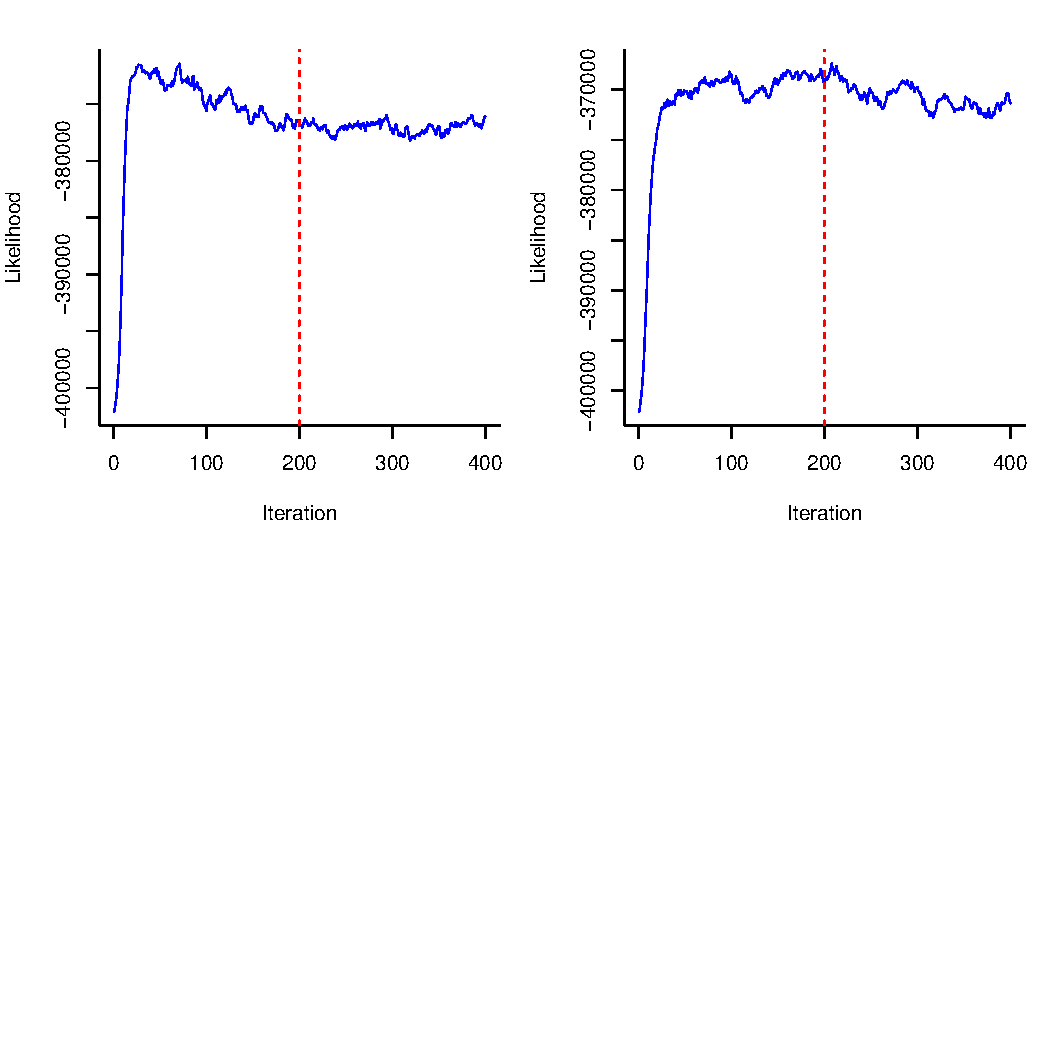
\includegraphics{vignettes/Diagnostic_Plots/diagnostics.likelihood.pdf}

\end{document}
